% Esta parte se enfoca en la factorizacion de matriz no negativa y como dividimos los audios mergeados a mano
\section{Aislando Instrumentos}

Analizamos la posibilidad de separar audios de distintos instrumentos por medio de la factorizaci\'on NMF. Como se vio antes esta factorizaci\'on nos descompone el sonido en una matriz tiene una base de vectores y en otra matriz de activaci\'on de michos vectores. Realizamos dos experimentos, uno combinando una guitarra con una flauta y luego otro combinando una trompeta con un violín. Notar que en ambos casos mezclamos una instrumento de viento con uno de cuerda.

\subsection{Modelo}

El modelo es similar el propuesto en la secci\'on anterior \ref{sec:modelo} . Utilizamos la factorizaci\'on NMF y luego reconstruimos el sonido con dicha factorizaci\'on.
 
\subsection{Experimentaci\'on}

\subsubsection{Guitarra y flauta}

Experimentamos anulando algunos de estos vectores e intentamos reconstruir los audios originales por separado. Tomamos un audio de Guitarra (nota LA en 4ta octava) y un audio de Flauta (nota RE en 5ta octava), los mezclamos en un mismo audio superponiendo el sonido.

\begin{figure}[h!]
    \centering
    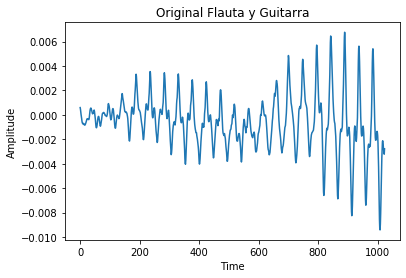
\includegraphics[height=60mm]{Content/Figures/separacion_original.png}
    \caption{Grafico del audio donde se mezclan Guitarra y Flauta}
\end{figure}

Luego separamos el audio en varios componentes usando la librer\'ia librosa para generar la matriz NMF. Con la matriz de factorizaci\'on fuimos anulando distintos vectores y reconstruyendo el audio con cada una de las nuevas matrices para luego quedarnos con aquellas matrices que tienen un mayor grado de correlaci\'on entre la matriz de factorizaci\'on de los audios por separado.
\\
\\
Con las nuevas matrices que tienen algunos vectores anulados pero que guardan mayor correlaci\'on con los sonidos originales reconstru\'imos el audio y los volvimos a graficar.

\begin{figure}[h!]
    \begin{subfigure}{0.5\textwidth}
        \centering
        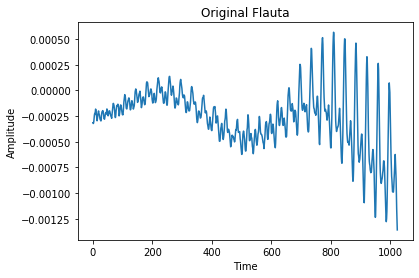
\includegraphics[height=60mm]{Content/Figures/separacion_audio1.png}
    \end{subfigure}
    \begin{subfigure}{0.5\textwidth}
        \centering
        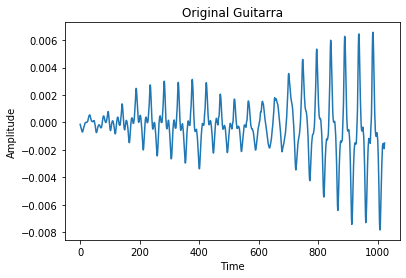
\includegraphics[height=60mm]{Content/Figures/separacion_audio2.png}
    \end{subfigure}
\end{figure}
\begin{figure}[h!]
    \begin{subfigure}{.5\textwidth}
        \centering
        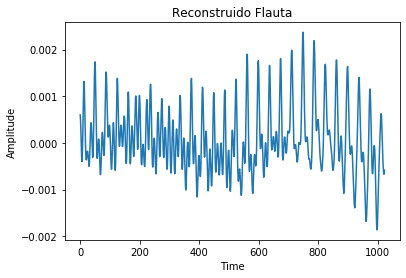
\includegraphics[height=60mm]{Content/Figures/separacion_reconstruccion_audio1.png}
    \end{subfigure}
    \begin{subfigure}{.5\textwidth}
        \centering
        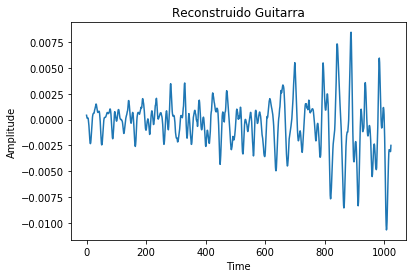
\includegraphics[height=60mm]{Content/Figures/separacion_reconstruccion_audio2.png}
    \end{subfigure}
\end{figure}

Como se puede observar, los audios reconstruidos mantienen un grado de similitud con los audios originales por separado. El sonido resultante de la reconstrucci\'on tambi\'en tienen un gran parecido con su audio original por separado a diferencia de otras tecnicas donde el audio reconstruido no guardaba mucha relaci\'on con el audio original.


Esta t\'ecnica podr\'ia ser util para la caracterizaci\'on de instrumentos como tambi\'en separaci\'on de audios. Con esta t\'ecnica no logramos separar audio en algunas de nuestras prueba indicando que esta t\'ecnica por si misma no es capaz de lograrlo. Sin embargo creemos que podr\'ia ser parte de t\'ecnicas m\'as avanzadas de caracterizaci\'on de sonido usando por ejemplo machine learning para detectar algunos aspectos del sonido.

\subsubsection{Violín y trompeta}
Al igual que en la sección anterior superpusimos los sonidos de dos instrumentos tocando una nota distinta. En este caso tomamos un violín y una trompeta. La nota correspondiente al sonido del violín es una D4, es decir octava prima de Re, en tanto la nota de la trompeta es una A4 lo que es lo mismo que una octava prima de La. La señal correspondiente a la mezcla se la puede ver en la siguiente figura:

\begin{figure}[h]
    \centering
    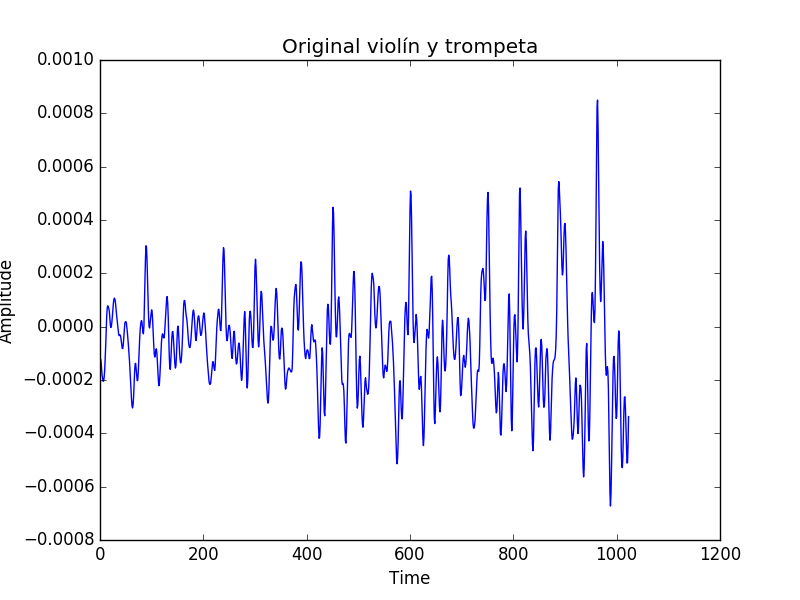
\includegraphics[height=60mm]{Content/Figures/orig_vio_trom.png}
    \caption{Grafico del audio donde se mezclan violín y trompeta}
\end{figure}

\newpage

Luego ejecutamos el script para separar la señal en las dos señales correspondientes a los instrumentos originales. Vale la pena aclarar que el script es exactamente el mismo que el que utilizamos para el experimento anterior.

\begin{figure}[h]
    \begin{subfigure}{0.5\textwidth}
        \centering
        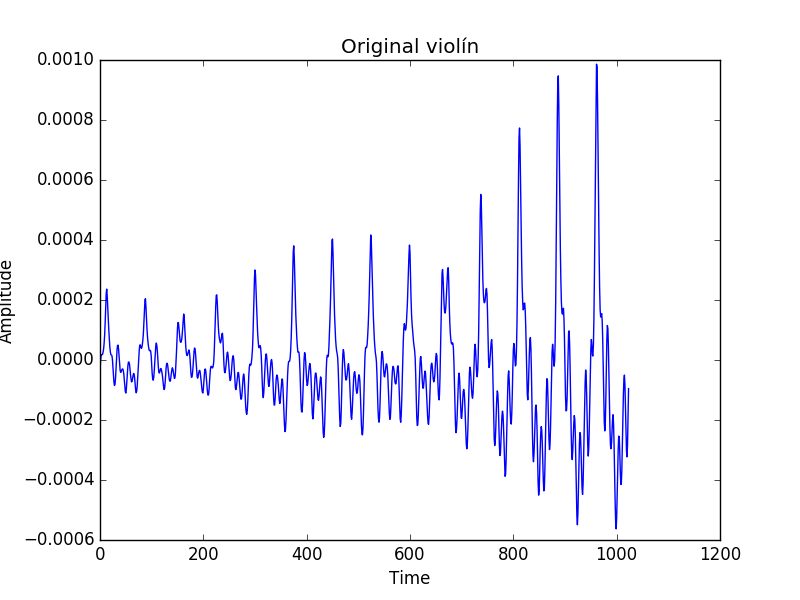
\includegraphics[height=60mm]{Content/Figures/orig_vio.png}
    \end{subfigure}
    \begin{subfigure}{0.5\textwidth}
        \centering
        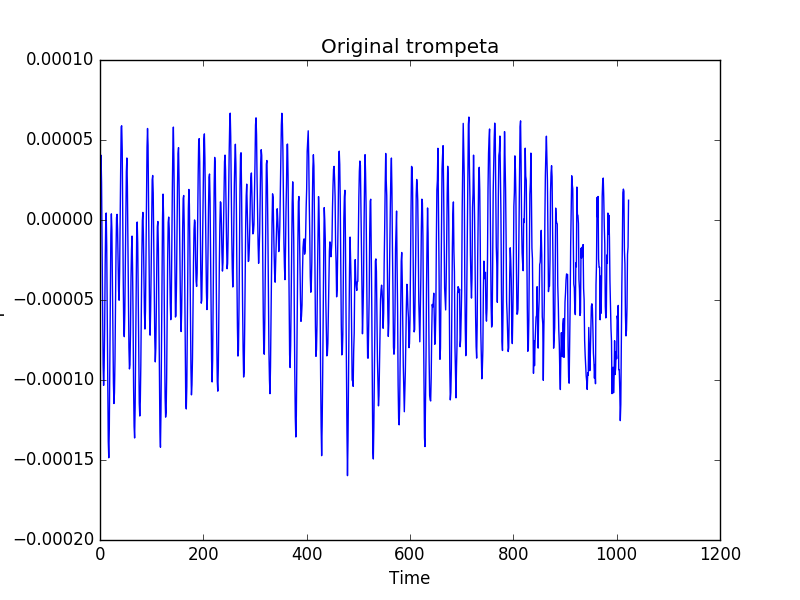
\includegraphics[height=60mm]{Content/Figures/orig_tromp.png}
    \end{subfigure}
\newline
    \begin{subfigure}{.5\textwidth}
        \centering
        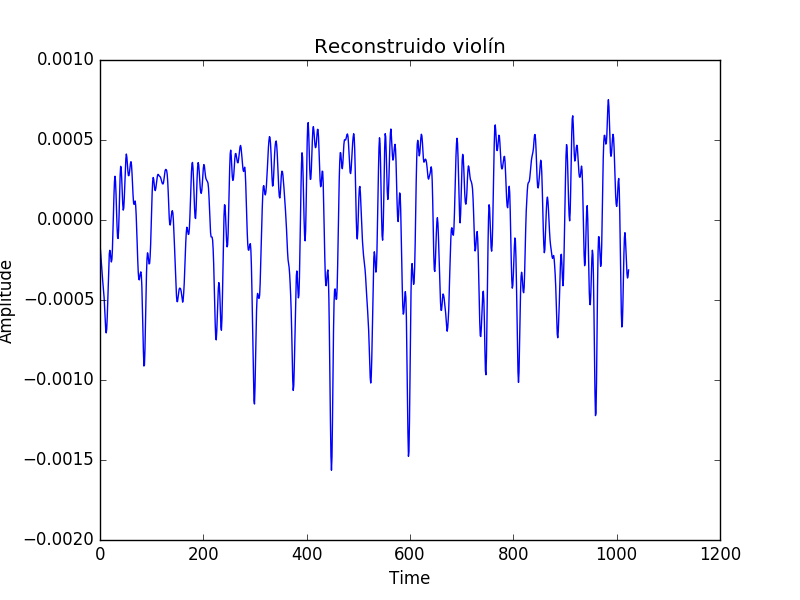
\includegraphics[height=60mm]{Content/Figures/recons_vio.png}
    \end{subfigure}
    \begin{subfigure}{.5\textwidth}
        \centering
        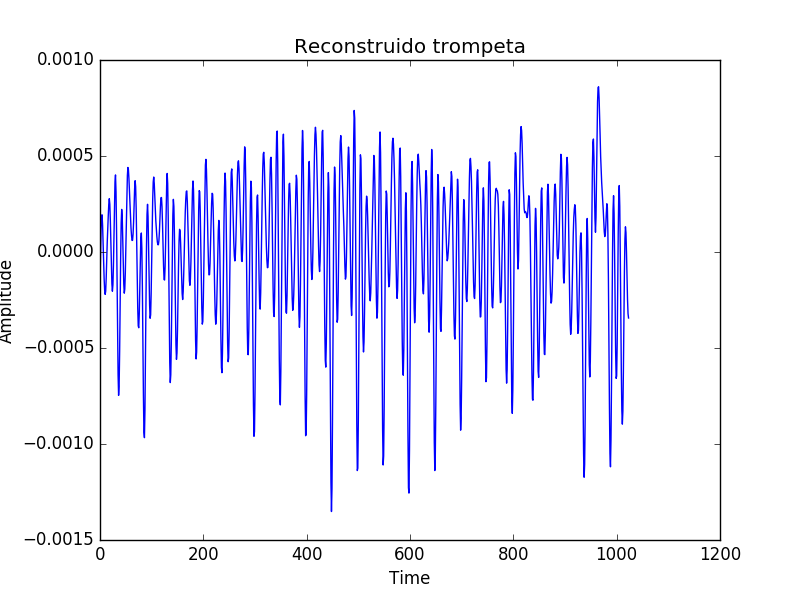
\includegraphics[height=60mm]{Content/Figures/recons_tromp.png}
    \end{subfigure}
\end{figure}

Como se puede apreciar en las figuras correspondientes a los audios originales la diferencia entre las señales es muy marcada pero en las versiones reconstruidas son similares. Además la trompeta se reconstruyó de manera satisfactoria mientras que el violín tiene bastantes diferencias. Por lo que podemos concluir que logró aislar correctamente la trompeta.
